\chapter{EXAMINATION OF PREVIOUSLY-EXISTING DP LIBRARIES}

The first goal of this Thesis is to examine previously existing programming libraries and APIs that provide the application of Differential Privacy to a dataset. This has been achieved by many companies, such as Google and IBM, but also from research programs like ARX that study the benefits of data privacy. We separate those implementations regarding their output. The possible outputs of a mechanism that adds D.P. to a dataset can be:
\begin{itemize}
    \item An answer to a query, in a private manner.
    \item An anonymized dataset, that meets the criteria of D.P.
\end{itemize}

In the first category, we can distinguish libraries such as Google's and IBM's, that have functions which if applied on a dataset, and given a specific query, can return a single answer.

In the second one, we can find libraries such as the ARX tool, that given a dataset and a group of privacy settings (such as the amount of noise to be inserted), produces an anonymized version of a dataset, that has obviously reduced information in comparison to the original one, but is usable by the final user.

In this chapter, we are going to test those libraries by providing different kinds of datasets, in order to determine the advantages and the disadvantages of each category.

We are going to conduct all of our testings using noise generated by the \textbf{Laplace Mechanism}, thus we must first define its theoretical behavior.



\section{The Laplace Mechanism}

The Laplace Mechanism is used widely in applications of Differential Privacy regarding \textbf{numerical queries}, which are actually functions that match a query to a number, or a vector of numbers, thus answering to it. The mechanism uses noise produced by the Laplace probabilistic distribution, which is equivalent to the query's sensitivity.

\subsection{Query Sensitivity}
The $l_1$ sensitivity of a query $f$, is defined as following:

\begin{align*}
    \Delta f = \max_{\{||x-y||_1 = 1\}} ||f(x) - f(y)||_1
\end{align*} where $x,y \in N^{|X|}$.

This quantity shows the effect by which a single participant's data can change in the worst case during the query $f$, and thus, the uncertainty that we must insert to to the response in order to protect them.

\subsection{The Laplace Distribution}
The Laplace Distribution with a scale $b$, is the distribution with probability density function: 
\begin{align*}
Lap(x|b) = \frac{1}{2b}exp(-\frac{|x|}{b})
\end{align*}

who's variance is $\sigma^2 = 2b^2$, and is actually a symmetric version of the exponential distribution.

\subsection{Use of Laplace in D.P.}

In order to be of use in our definition, the scale of the noise will be calibrated to the sensitivity of the query $f$, divided by epsilon. Thus, the noise used will be drawn from

\begin{align*}
Lap(\frac{\Delta f}{\epsilon})
\end{align*}

Of course, many other probabilistic distributions can be used to ensure differential privacy, but during our testings we prefer to use Laplace.

\section{Query Answering Libraries}

We are going to begin by testing libraries that belong in the first category, and specifically the \textbf{IBM's diffprivlib}, which is written in python, and is publicly available \href{https://github.com/IBM/differential-privacy-library}{here}. The library includes a host of mechanisms, the building blocks of differential privacy, alongside a number of applications to machine learning and other data analytics tasks. We are going to focus our testings in the simple queries, such as the \textbf{mean value}, the \textbf{extreme values} and the \textbf{histograms} of a numerical dataset. The library consists of three modules:

\begin{itemize}
    \item \textbf{Mechanisms}, as known from the theoretical foundations of D.P.
    \item \textbf{Models}, especially machine learning models, that will not concern us during this thesis
    \item \textbf{Tools} that will allow us to apply D.P. in datasets.
\end{itemize}

We are going to use the tools available, in order to apply differential privacy in a dataset of our own, guided of course by the mechanisms provided by diffprivlib. First, we are going to take a look at the dataset that we are going to use going forward.


\subsection{Setup of the mechanism}

The first step in order to test the library, is to setup the mechanism by defining its properties and parameters. 

\subsubsection{Bounds' Definition}

One of the most important aspects for us if we want to apply DP algorithms, is to define the bounds, i.e. the range that a variable can be in. It would be very convenient in our case to just take the tuple of the smallest and the largest value in the column that we are interested in. However, in the real world, the person who asks the queries is not supposed to know this info about the dataset. Thus, since a solution is not provided by the library, we must define our own bounds by guessing the lowest and the highest values in the fields that we want to examine. 

Thus, the user must have somewhat of a previous knowledge regarding the dataset, in order to decide the minimum and maximum value. Those values do not need to be precise, although the more close they are to real ones, the best the protocol will function. At the same time, we must be sure that during our selection we do not leave some of the dataset's values outside of the bounds, as they will be ignored in the final results. 

We are considering fees for surgeries in our example, thus a logical lower bound would be 0\$ (surgeries could be done pro bono too!), and an upper bound would be 1 million dollars. Either way, we are trying to be extreme with our picks, in order to not find ourselves in the unfortunate situation that a value taken into consideration by the DP query would be out of bounds.

\subsubsection{Privacy Budget}

In this form of D.P., someone trying to breach the users' privacy, could theoretically ask an infinite number of questions, and thus each time gain more and more information about their private data. This is not covered by the definition of D.P., however it is not acceptable. In the same manner, an untrusted user of the library could ask the same question many times, aiming to determine how much noise is added each time, in order to find out the actual answer to the query, as the way that the noise is drawn is already known.

In order to eliminate this problem, a special parameter call the \textbf{privacy budget} is implemented. The library offers the ability to initialize this budget before asking any queries. During the queries, this budget is each time decreased, according to how much data the answer to the question reveals. For example, the answer to the "mean value of the charges for a surgery", costs less than the answer to the "histogram values of heart transplant surgeries in the West coast".

This parameter is implemented by the library as the budget accountant. This variable tracks the privacy spent, so that our system is not left exposed after lots of "expensive queries". The system will allow someone to ask one question that uses the whole privacy budget, or a series of questions whose total impact is less or equal to the initial budget.

\subsection{Testings' goal}

When applying D.P. mechanisms to our data, we provide the privacy settings of our choice (epsilon variable), and obtain an answer to each of our questions. Thus, in our testings, our goal is to \textbf{determine the accuracy of the answers}, given a specific $\epsilon$, or some other settings, and comparing them to the true answer, using some metrics. Those metrics are different for each query type. In this section we are going to focus on two types of queries: statistical, and histograms.

\subsection{General techniques}
In each one of our following testings, we are going to run the query \textbf{many times}. As we already know, D.P. relies on probabilistic algorithms that can some times produce extreme results. This may be rare, but we want our testings and conclusions to be accurate. So, we are going to run each query 100 times, and return as a result the mean value of those runs.

\subsection{Statistical Queries}

The first type of queries that we are going to test are those that answer questions like "What is the mean cost of a surgery?", or "What is the largest fee paid by medicare for a transplant?", known as statistical queries. 

\subsubsection{Metrics used}

In the case of statistical queries, their answer is usually a real number, so in order to check their alteration with the true answer, we are going to take into account the \textbf{absolute difference between the truth and the query answer}. 

\subsubsection{The identity of the testing Dataset}

The dataset chosen to test the library, is the publicly available "Surgery Charges Across the U.S.", that contains many different kinds of surgeries in a plethora of different hospitals. Our goal is to protect each hospital's data when it comes down to a specific surgery, while helping a patient choose one, depending on the charges that can be found all over the United States. The data provided in this dataset, is going to help a potential patient balance his need of top care, and the need to spend less money. The columns contained in the dataset are:

\begin{itemize}
    \item Surgery code and definition
    \item Provider hospital name
    \item Provider city
    \item Average total payments
    \item Average medicare payments
\end{itemize}

We are going to focus on the last two columns, in order to approximate the charges of a surgery. The above table gives us an image of the containers of the dataset.

The dataset contains a total of 200,000 entries, a more than satisfying number for running D.P. algorithms.

\begin{table}[!htb]

    \caption{"Surgery Charges Across the U.S." dataset columns}
    \label{numbers}

    \begin{tabular}{| c | c | c | c | c| c |}
      \hline 
      ID & Surgery Type & Hospital Name & Hospital City & Total & Medicare \\
      \hline
      1 & TRANSPLANT & MAYO CLINIC & PHOENIX & \$240422.80 & \$133509.55\\
      \hline
      2 & ECMO &  GROSSMONT HOSP & LA MESA & \$193617.86 & \$192003.43 \\
      \hline
      3 & CRANIOTOMY & STANFORD HOSP &  STANFORD & \$32597.87 & \$29347.12  \\
      \hline
    \end{tabular}

\end{table}

\subsubsection{General Dataset Utilities Queries}

Our first experiment is just to ask for some of the utilities of the dataset, and specifically its cost column: the \textbf{mean value}, the \textbf{variance}, the \textbf{sum} and the \textbf{standard deviation} values of the surgeries' cost. 

All of those queries can be executed using the following command (specifically for the mean value query):
\bigskip

\begin{lstlisting}[language=Python]
mean_with_dp = dp.tools.mean(df["Average_Total_Payments"].tolist())
\end{lstlisting}
\bigskip

where the dataframe column is the one containing the cost of each surgery.

By running the above mentioned queries, we got the following results:

\begin{table}[!htb]
    \centering
    \caption{General Queries results for Surgeries Dataset}
    \label{numbers}

    \begin{tabular}{| c | c | c |}
      \hline 
      Query & True answer & Private Answer \\
      \hline
      Mean value & 13168.5 & 13167.3 \\
      \hline
      Sum & 262754253.1 &  262935459.3 \\
      \hline
      Variance & 262754253.1 & 261940796.5\\
      \hline
      Standard Deviation & 18855.1 & 25825.0\\
      \hline
    \end{tabular}

\end{table}


The answers are almost perfect, for example on the mean value, considering that the cost is thousands of dollars, and the error is just 1 dollar. The simplicity of the query just lies to the following instruction:

However, this is just a simple example, executed only once, hence it can not provide us with safe conclusions for the library. In order to do so, we are going to run more complicated examples moving forward.

\subsubsection{Lowering the Dataset size}

As we mentioned above, the entries that the dataset contains are a very large number, and we know as a fact that D.P. functions well when this is the case. How is the library going to respond though if the dataset size is smaller? We are going to run for 4 different values of epsilon, and get the results for an increasing number of entries, starting from 10, and moving to 2000. Thus, the X axis of each plot represents the increasing dataset size, the Y axis the accuracy error, and each plot has a title of the epsilon setting used for the measurements. We can see the results in the Figure 3.1 below.

\begin{figure}[!htb]\centering
    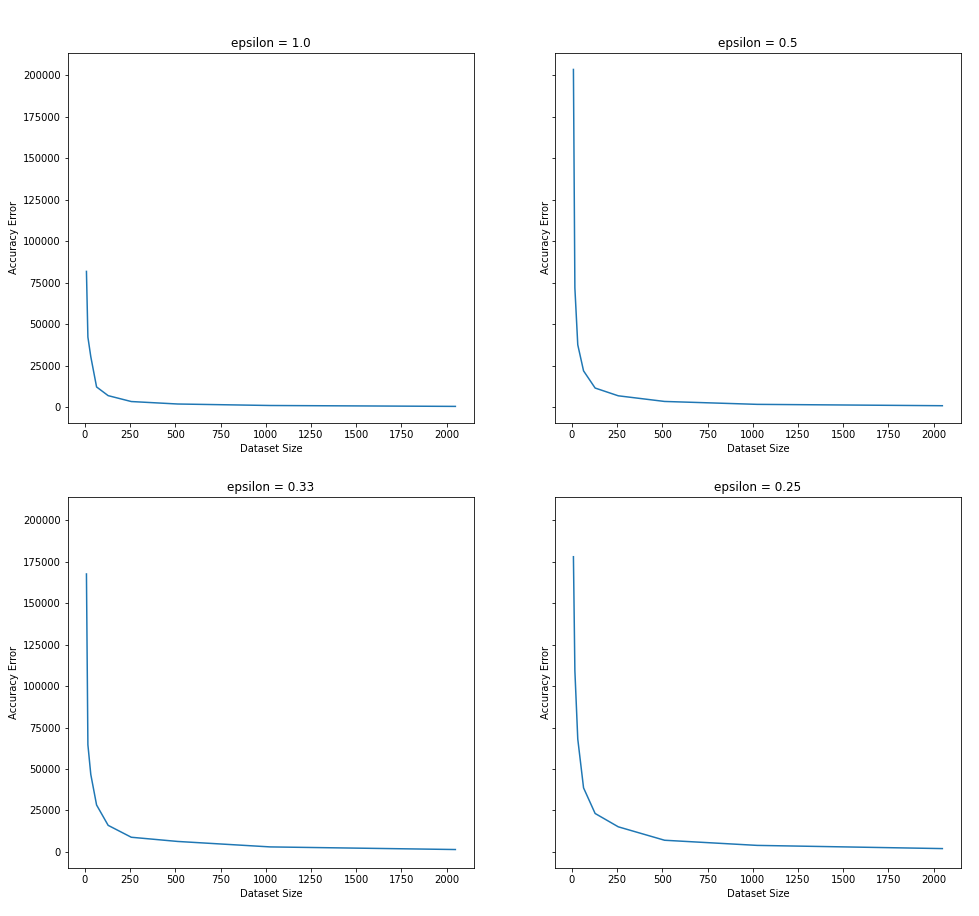
\includegraphics[width=1\textwidth]{images/increasing_ds_size.png}
    \caption{Accuracy Error for Increasing Dataset Sizes}
\end{figure}


By observing the plots, we can make a couple of conclusions:

\begin{itemize}
    \item \textbf{The smaller the epsilon gets, the bigger the accuracy error in the case of small datasets.} This, according to the definition makes sense, because small epsilon indicates higher privacy, thus for small datasets it can mean lower accuracy, due to the high amount of noise added.
    \item \textbf{The accuracy error stabilizes near 0 as the size of the dataset gets over 1000 entries.} Of course, depending to the epsilon value, this point could be earlier in the dataset sizes, as we observe for $\epsilon = 1$. This again lays in the above mentioned property of the definition.
\end{itemize}

\subsection{Histogram Queries}


